% sage_latex_guidelines.tex V1.10, 24 June 2016

\documentclass[Afour,sageh,times]{sagej}
\usepackage{moreverb,url}
\usepackage[colorlinks,bookmarksopen,bookmarksnumbered,citecolor=red,urlcolor=red]{hyperref}
\newcommand\BibTeX{{\rmfamily B\kern-.05em \textsc{i\kern-.025em b}\kern-.08em
T\kern-.1667em\lower.7ex\hbox{E}\kern-.125emX}}

% customizations
\usepackage[super]{nth}
\usepackage[inline]{enumitem}
\usepackage{moreenum}
\usepackage{tabulary}
\usepackage{tabu}
\usepackage{booktabs}
\usepackage{array}
\usepackage[super]{nth}
\usepackage{listings}
\usepackage{float}
\usepackage{tikz}
\usepackage{upquote}
\usepackage{graphicx}
\usepackage{epstopdf}
\usepackage{tabularx}
\newcolumntype{Y}{>{\raggedright\arraybackslash}X}
\newcommand{\ra}[1]{\renewcommand{\arraystretch}{#1}}

% special characters
\usepackage{gensymb}
\usepackage{amssymb}
\usepackage{pifont}
\newcommand{\cmark}{\ding{51}}
\newcommand{\xmark}{\ding{55}}

% ---------------------------- METADATA ---------------------------- 

\def\volumeyear{2017}
\begin{document}
\runninghead{Harmon et~al.}
\title{Tangibly modeling landscapes}
%\title{Tangible Landscape}
%\title{Tangible Landscape Architectural Modeling}
%\title{Tangible Landscape Modeling}
\author{Brendan A Harmon\affilnum{1,2}, Anna Petrasova\affilnum{1}, Vaclav Petras\affilnum{1}, Helena Mitasova\affilnum{1}, and Ross Meentemeyer\affilnum{1}}
\affiliation{\affilnum{1}Center for Geospatial Analytics, North Carolina State University, USA\\
\affilnum{2}College of Design, North Carolina State University, USA}
\corrauth{Brendan A Harmon, 
Center for Geospatial Analytics,
North Carolina State University,
Raleigh, NC 27615, USA.}
\email{brendan.harmon@gmail.com}

% ---------------------------- ABSTRACT ---------------------------- 

\begin{abstract}
We present Tangible Landscape 
-- a technology for rapidly and intuitively designing landscapes
informed by geospatial modeling, analysis, and simulation.
%
Tangible Landscape is a tangible interface powered by a geographic information system 
that gives 3D spatial data an interactive, physical form so that 
users can naturally sense and shape it.
%
It couples a physical and a digital model of a landscape
through real-time cycles of 
physical manipulation, 3D scanning, spatial computation, and projected feedback.
% 
Natural 3D sketching and real-time analytical feedback should aid
landscape architects in the design of high performance, process-based landscapes.
%
We conducted a series of studies to assess the effectiveness of 
tangible modeling for landscape architects.
%
Landscape architecture students, academics, and professionals 
were given a series of fundamental landscape design tasks 
-- topographic modeling, cut-and-fill analysis, and water flow modeling. 
%
Their performance was assessed using both qualitative and quantitative methods.
%
With tangible modeling the participants
effectively modeled topography and water flow 
producing more accurate models 
that better represented morphological features 
than they did with either digital or analog, hand modeling.
%
When tangibly modeling
they used a rapid, iterative process informed by geospatial analytics 
that enhanced their performance.  
\end{abstract}

\keywords{Human-computer interaction, tangible interfaces, embodied cognition, geospatial modeling, topographic modeling, hydrological modeling}

\maketitle

% ---------------------------- INTRO ---------------------------- 

\section{Introduction}

% GIS IN LANDSCAPE ARCHITECTURE
Landscape architects use 
geographic information systems (GIS) to map and analyze landscapes
and computer aided design (CAD) software % 3D modeling software
to computationally represent and design landscapes.
%
While GIS can quantitatively model, analyze, simulate, and visualize 
complex spatial and temporal phenomena,
these systems can be unintuitive, challenging to use, and creatively constraining
due to the complexity of the software, 
the complex workflows, 
and the limited modes of interaction and visualization 
\cite{Ratti2004}. 
%
Due to the complex, time consuming workflows 
needed to link geospatial analysis with computer aided design 
GIS tends to play a limited, often preliminary role in the creative design process.
%
While GIS has been used extensively in landscape planning 
to model scenarios \cite{Steinitz2004,Baker2004,Steinitz2012},
in landscape architecture
it is primarily used for preliminary research and mapping.
%
If, however, geospatial analysis, modeling, and simulation
could be seamlessly integrated into the creative design process 
then designers could rapidly develop design ideas
while quantitively testing them. 
%
In such a rapid, fluid creative process
the rigorous testing of design concepts 
with quantitive measures of performance 
could drive the development of new concepts.
%
Simulation for example could inspire ideation 
linking designed form with environmental processes. 

% TANGIBLES
When using a graphical user interface (GUI) 
-- the paradigmatic mode of interaction for both CAD and GIS --  
intention is translated from physical input 
using devices like a mouse and keyboard 
to digital data rendered visually as text and graphics. 
%
Positing that graphical interaction is unintuitive
because of this disconnect between 
intention, physical action, and purely visual feedback,
researchers have been developing tangible user interfaces 
to give digital data interactive physical form 
\cite{Dourish2001,Ishii2008}. 
%
Theoretically tangible interfaces should embody cognition 
-- grounding higher cognitive processes in bodily experience --
by enabling users to kinaesthetically sense and interact with digital data
\cite{Kirsh2013}.
%
Tangible, embodied interaction should be highly intuitive 
since it 
uses existing motor schemas,  
offloads cognitive work onto the body,
and seamlessly connects intention, action, and feedback.

% TANGIBLES FOR LANDSCAPE ARCHITECTURE
The MIT Media Lab developed two prototypes 
-- Illuminating Clay and SandScape -- 
that coupled a physical and digital model of a landscape
through a cycle of 3D scanning, geospatial computation, and projection
to combine the affordances of intuitive sculpting by hand
with quantitative geospatial analysis \cite{Piper2002a}. 
%
These systems were designed to 
'streamline the landscape design process 
and result in a more effective use of GIS, 
especially when distributed decision-making and discussion 
with non-experts are involved' \cite{Ratti2004}.
%
Recent advances in sensors and computer vision
have fueled the development of 
%new tangible interfaces including systems 
systems for tangibly modeling landscapes such as 
Efecto Mariposa \cite{Vivo2011} and
the Augmented Reality Sandbox \cite{Kreylos2012}, 
Sedimachine \cite{Cantrell2014}, and
the Rapid Landscape Prototyping Machine \cite{Robinson2014}.

\subsection{Tangible Landscape}
Inspired by Illuminating Clay, 
the Tangible Geospatial Modeling System \cite{Mitasova2006,Tateosian2010}, 
and the Augmented Reality Sandbox, 
we have develop Tangible Landscape 
-- a tangible interface for geospatial modeling
powered by an open source GIS \cite{Petrasova2015}. 
%
% TL premise: algorithmic design of landscapes
% Conceptually Tangible Landscape is meant to... 
%
With Tangible Landscape
designers can sculpt a terrain model in polymeric sand,
and can digitize points, areas, and volumes by placing 
color-coded markers, patches of felt, or building blocks. 
%
These interactions are captured by a Kinect sensor, 
processed in GRASS GIS, 
and the resulting geospatial computations
are projected back onto the physical model, 
all in real-time (Fig.~\ref{fig:system_diagram}).
%
The geospatial data can also be automatically
3D modeled and rendered in Blender 
on a monitor or head-mounted display
so that designers can 
immersively explore different views \cite{Tabrizian2016}.
%
For example
as users sculpt topography,
simulated water flow can be projected back onto the model in real-time
so that they understand how they are affecting 
physical processes in landscape.
Then as they draw planting areas 
using a laser pointer or patches of colored felt,
the trees can be rendered in 3D on a display %. 
%As they place markers to designate waypoints on a trail,
%the optimal walking route can be computed and projected onto the model
%along with charts showing metrics like distance and slope
(Fig.~\ref{table:tl_demo}). 

Tangible Landscape 
is unique since it powered by a GIS
with extensive libraries for geospatial computation
and has a wide range of real-time interactions including 
3D sculpting, 3D sketching, color recognition, and object recognition.
%
Given its versatility 
there are many possible design applications
including terrain modeling, hydrological modeling, flood prevention,
trail planning, viewshed analysis, and planting design. 

% TL DIAGRAM
\begin{figure}
    \begin{center}
        \includegraphics[width=0.45\textwidth]{images/diagrams/rendered_diagram.png}
        \caption{Tangible Landscape: a real-time cycle of 3D scanning, geospatial computation and 3D modeling, and 3D rendering and projection.}
        \label{fig:system_diagram}
    \end{center}
\end{figure}

% TL DEMO
\begin{table*}
\caption{Collaboratively sculpting topography to create lakes, drawing trees with a laser pointer, and visualizing with 3D renderings.} %Source: \cite{Tabrizian2016}.
\ra{1.3}
\begin{tabular}{m{0.49\textwidth} m{0.49\textwidth}}
\toprule
\multicolumn{1}{c}{Sculpting}  & \multicolumn{1}{c}{Drawing and visualization}\\
\midrule
%
\includegraphics[width=0.49\textwidth]{images/immersive/sculpting_lakes_2.png} &
\includegraphics[width=0.49\textwidth]{images/immersive/drawing_trees_1.png}\\
%
\includegraphics[width=0.49\textwidth]{images/immersive/sculpting_landforms_2.png} &
\includegraphics[width=0.49\textwidth]{images/immersive/drawing_trees_2.png}\\
%
\includegraphics[width=0.49\textwidth]{images/immersive/sculpting_landforms_3.png} &
\includegraphics[width=0.49\textwidth]{images/immersive/trees_with_oculus_1.png}\\
%
\bottomrule
\end{tabular}
\label{table:tl_demo} 
\end{table*}

%% TL DEMO V2
%\begin{table*}
%\caption{Sculpting topography to create lakes, 
%drawing trees with a laser pointer, 
%and visualizing with 3D renderings.} 
%\ra{1.3}
%\begin{tabular}{m{0.49\textwidth} m{0.49\textwidth}}
%\toprule
%\multicolumn{1}{c}{Sculpting and views}  & \multicolumn{1}{c}{Drawing and immersion}\\
%\midrule
%%
%\includegraphics[width=0.49\textwidth]{images/immersive/tl_vr_demo_2.jpg} &
%\includegraphics[width=0.49\textwidth]{images/immersive/tl_vr_demo_8.jpg}\\
%%
%\includegraphics[width=0.49\textwidth]{images/immersive/tl_vr_demo_4.jpg} &
%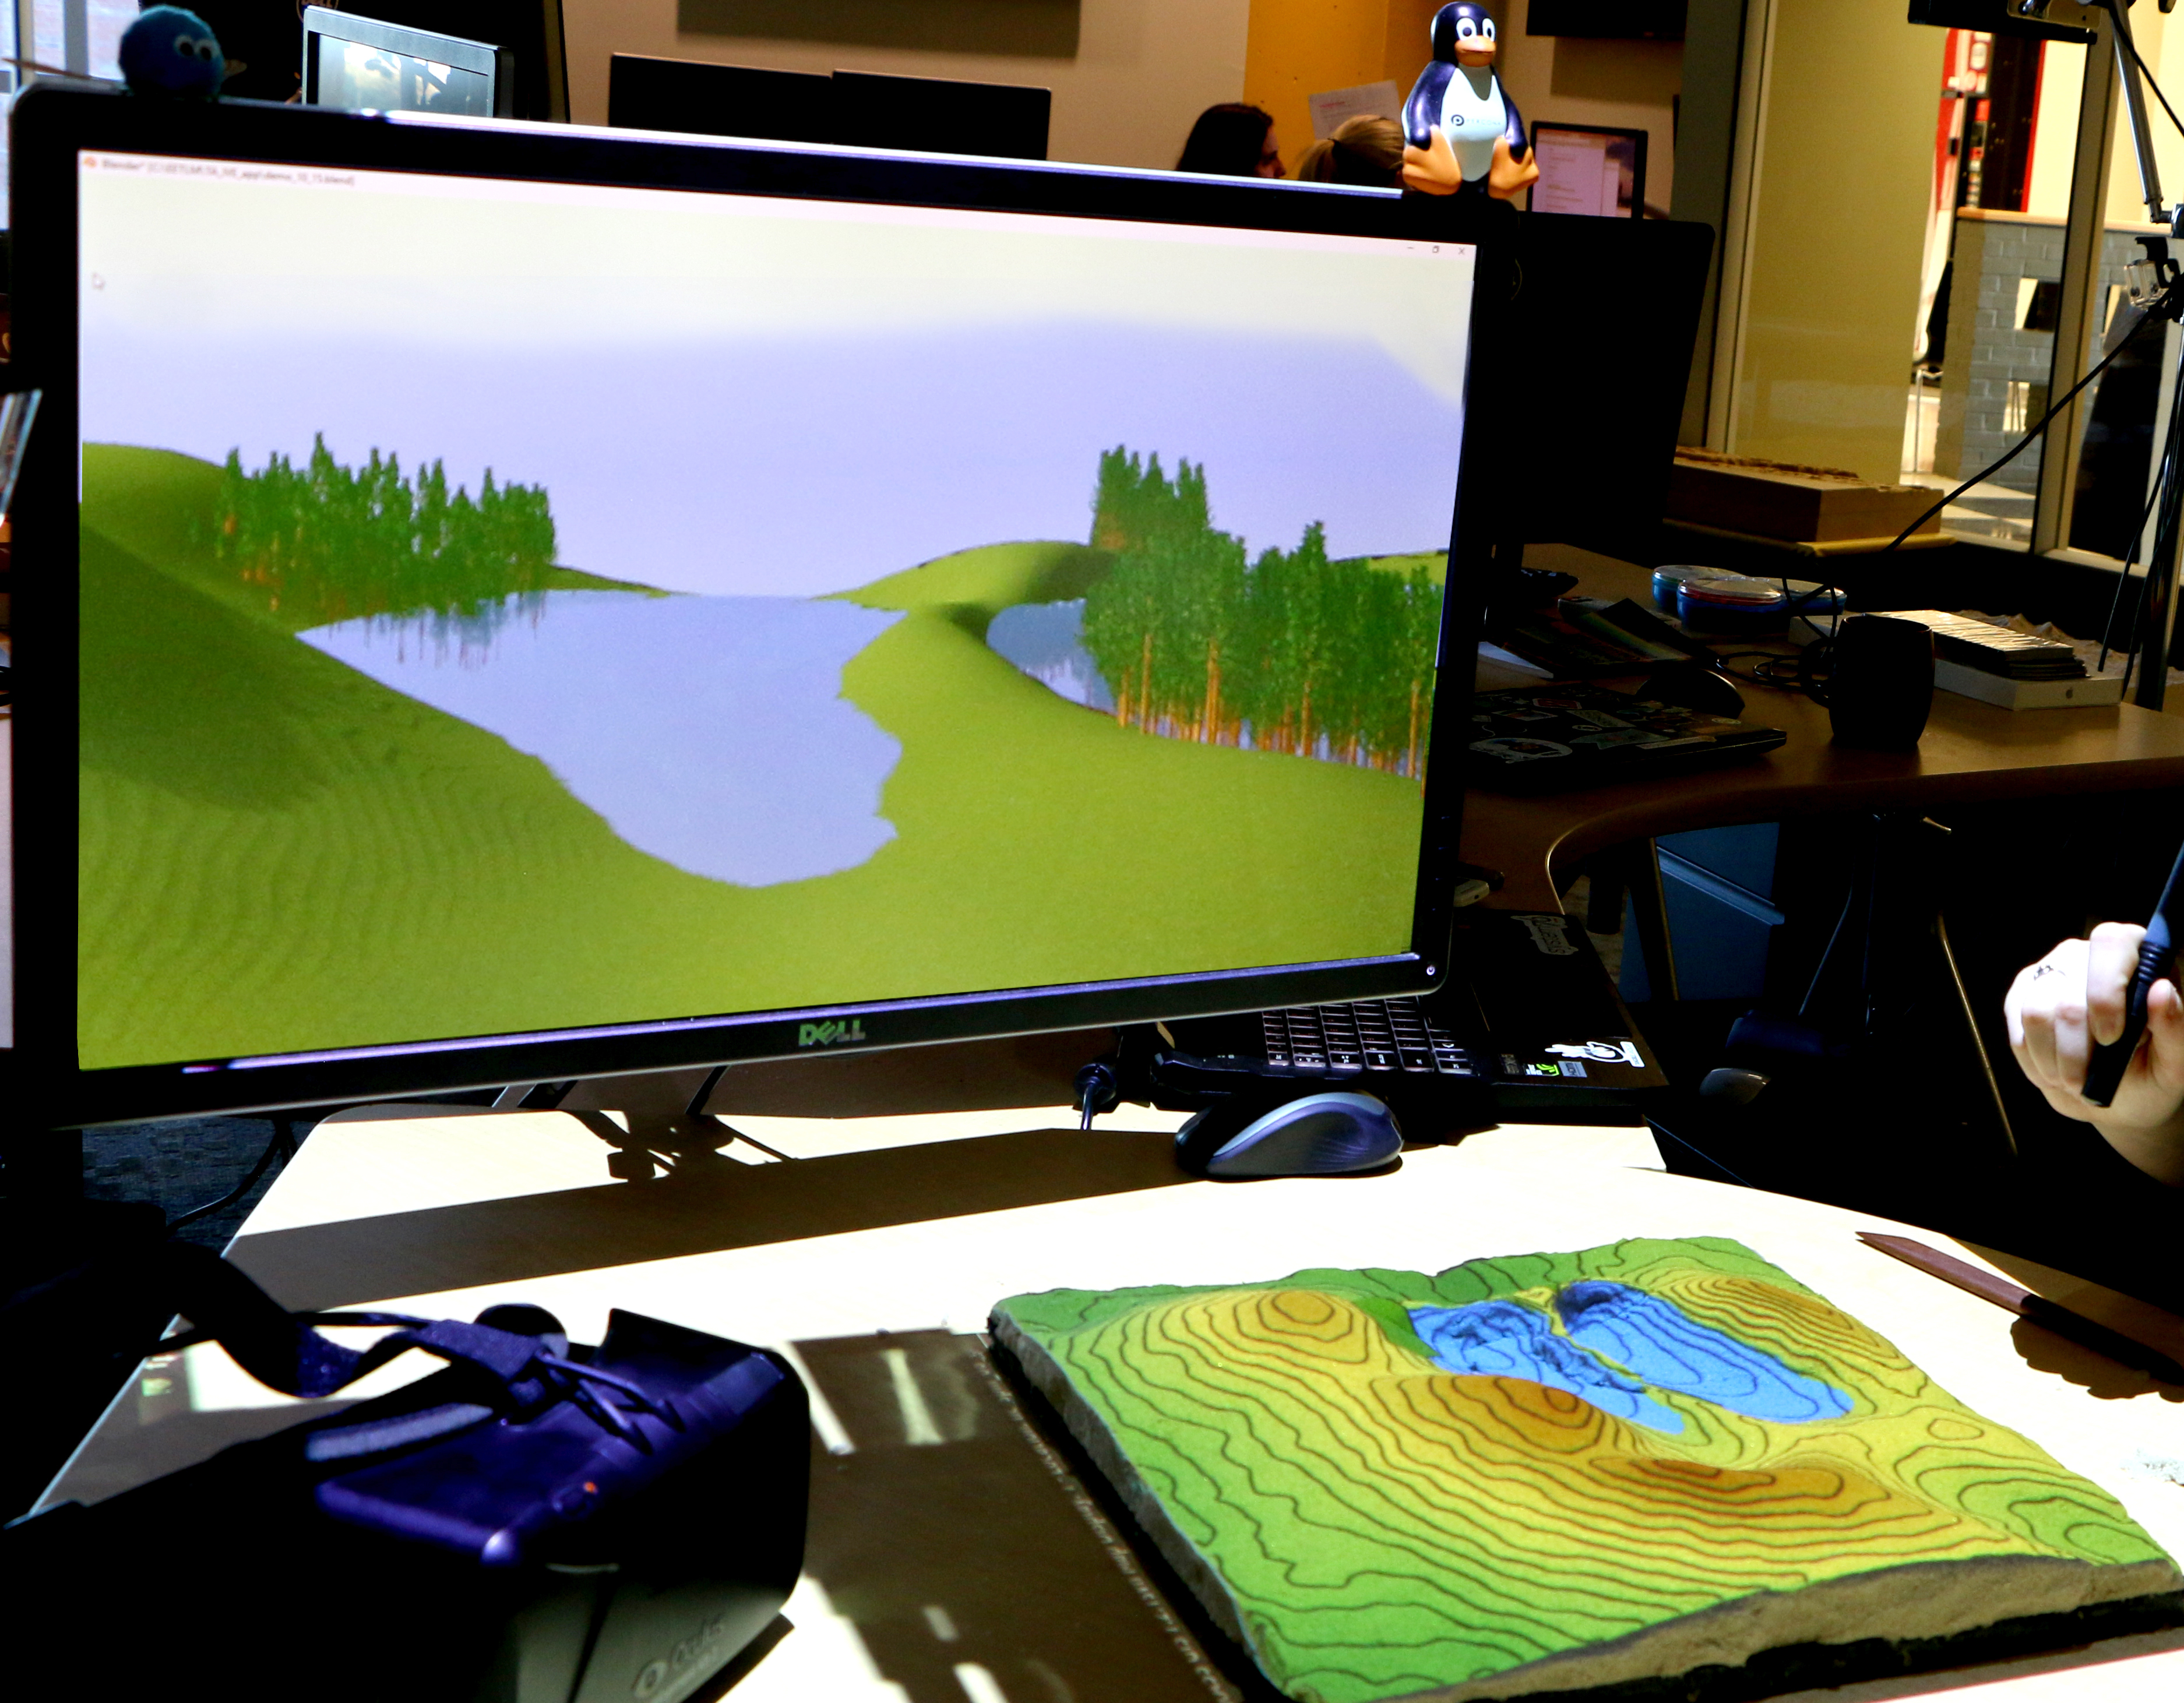
\includegraphics[width=0.49\textwidth]{images/immersive/tl_vr_demo_9.jpg}\\
%%
%\includegraphics[width=0.49\textwidth]{images/immersive/tl_vr_demo_5.jpg} &
%\includegraphics[width=0.49\textwidth]{images/immersive/tl_vr_demo_10.jpg}\\
%%
%\bottomrule
%\end{tabular}
%\label{table:tl_demo} 
%\end{table*}

% RESEARCH QUESTIONS
\subsection{Research objectives}
Many of the theoretical underpinnings of tangibles 
remain unproven and unexplored. 
Do current approaches to tangible, embodied interfaces
really work as theorized? 
Can designers really model more intuitively and 
design more effectively with tangibles?
And how do tangibles mediate the design process?
%
In order to assess the effectiveness 
of tangible modeling for landscape architects 
we conducted a series of user studies
assessing how well participants performed
basic landscape design tasks 
-- topographic modeling, cut-and-fill analysis, and water flow modeling --
using Tangible Landscape.\\

Our research objectives were to:
%
\begin{itemize}
% Performance
\item Assess how well landscape architects could perform basic design tasks using
a tangible interface for landscape modeling
% Process
\item Study how tangible interaction mediated
landscape architects' design process
\end{itemize}

\clearpage

% ---------------------------- TOPOGRAPHIC ---------------------------- 

\section{Topographic modeling}

% describe topographic modeling and its role in landscape architecture
% how is it typically done?
% how is it done by hand - clay models, contours models, etc.
% brief discussion of digital methods and software 

%Grading -- earth moving --
%and thus
%topographic modeling are an important part of landscape architecture

We conducted a topographic modeling experiment 
comparing 
digital 3D modeling with Rhinoceros, 
analog modeling by hand, 
and tangible modeling with Tangible Landscape. 

%% digital
%Digital modeling with a GUI affords precise transformations and
%dynamic modes of visualization such as 
%3D orbiting, zooming, and ray traced shading,
%but is not embodied.
%% analog
%Theoretically analog modeling -- modeling by hand or with tools -- 
%should be embodied, 
%affording subconscious, kinaesthetic sensing and manipulation of form. 
%By sensing form subconsciously with the body
%users should have more cognitive resources for critiquing their work 
%and strategizing their next moves. 
%% 
%tangible modeling 
%couples digital mapping with physical modeling.
%Theoretically it should combine affordances of both -- 
%enabling enriched visualization and physical sensing and manipulation -- 
%to offer more feedback.
%While more feedback may help users 
%better assess and critique their performance 
%so they can strategize their next moves,
%too much feedback may be a cognitive overload 
%resulting in distraction, frustration, and demotivation. 
%Physical sensing and manipulation, however, should offload 
%some of this cognitive work onto the body.
%









\subsection{Methods}













%Training for digital 3D modeling: \\
\noindent \url{https://youtu.be/dSyrHAuu698}

%Digital 3D modeling with Rhinoceros: \\
\noindent \url{https://youtu.be/vA1xwMSaGV4}

%Analog 3D modeling: \\
\noindent \url{https://youtu.be/STYHUHNaWdY}

%Tangible modeling: \\
\noindent  \url{https://youtu.be/1uEvzMJWh_E}



% See Supplemental Material for more detailed methodolgy

\subsection{Results}

\begin{figure*}%[h]
\begin{center}
\resizebox {\textwidth} {!} {\begin{tikzpicture}[grow = right,
	level 1/.style={sibling distance=12 em},
	level 2/.style={sibling distance=6 em},
	level distance = 14em,
	every node/.style = {shape=rectangle, 
		rounded corners,
		draw, 
		font=\footnotesize\sffamily,
		align=center,
		top color=white,
		bottom color=white}]
\node {Participants \\ 
	\includegraphics[width=0.08\textwidth]{images/render_3d/participants/mean_dem_1.png}
	\includegraphics[width=0.08\textwidth]{images/render_3d/participants/mean_dem_2.png}
	\includegraphics[width=0.08\textwidth]{images/render_3d/participants/mean_dem_3.png} \\
	\makebox[0.08\textwidth][c]{\scriptsize Digital}
	\makebox[0.08\textwidth][c]{\scriptsize Analog}
	\makebox[0.08\textwidth][c]{\scriptsize Tangible}
	}
	child { node {Students \\ 
		\includegraphics[width=0.08\textwidth]{images/render_3d/students/mean_dem_1.png}
		\includegraphics[width=0.08\textwidth]{images/render_3d/students/mean_dem_2.png}
		\includegraphics[width=0.08\textwidth]{images/render_3d/students/mean_dem_3.png}
		}
		child { node {Landscape architecture \\ 
			\includegraphics[width=0.08\textwidth]{images/render_3d/landscape_students/mean_dem_1.png}
			\includegraphics[width=0.08\textwidth]{images/render_3d/landscape_students/mean_dem_2.png}
			\includegraphics[width=0.08\textwidth]{images/render_3d/landscape_students/mean_dem_3.png}
			}
			}
		child { node {GIS \\ 
			\includegraphics[width=0.08\textwidth]{images/render_3d/gis_students/mean_dem_1.png}
			\includegraphics[width=0.08\textwidth]{images/render_3d/gis_students/mean_dem_2.png}
			\includegraphics[width=0.08\textwidth]{images/render_3d/gis_students/mean_dem_3.png}
			}
			}
		}
	child { node {Professionals \\ 
		\includegraphics[width=0.08\textwidth]{images/render_3d/professionals/mean_dem_1.png}
		\includegraphics[width=0.08\textwidth]{images/render_3d/professionals/mean_dem_2.png}
		\includegraphics[width=0.08\textwidth]{images/render_3d/professionals/mean_dem_3.png}
		}
		child { node {3D novices \\ 
			\includegraphics[width=0.08\textwidth]{images/render_3d/3d_novices/mean_dem_1.png}
			\includegraphics[width=0.08\textwidth]{images/render_3d/3d_novices/mean_dem_2.png}
			\includegraphics[width=0.08\textwidth]{images/render_3d/3d_novices/mean_dem_3.png}
			}
			}
		child { node {3D experts \\ 
			\includegraphics[width=0.08\textwidth]{images/render_3d/3d_experts/mean_dem_1.png}
			\includegraphics[width=0.08\textwidth]{images/render_3d/3d_experts/mean_dem_2.png}
			\includegraphics[width=0.08\textwidth]{images/render_3d/3d_experts/mean_dem_3.png}
			}
			}
};
\end{tikzpicture}
}
\caption{Pairwise comparison of the mean digital elevation models by category of participants}
\label{fig:comparison}
\end{center}
\end{figure*}

% See Supplemental Material for more detailed comparison

%% ---------------------------- TOPOGRAPHY ---------------------------- 
\begin{table*}[h]
\small\sf\centering
\caption{Topographic experiment: maps of raster statistics and geospatial analyses draped over 3D topography for all participants.}
\ra{1.3}
\begin{tabular}{m{0.16\textwidth} m{0.18\textwidth} m{0.18\textwidth} m{0.18\textwidth} m{0.18\textwidth}}
\toprule
& \multicolumn{1}{c}{Reference} & \multicolumn{1}{c}{Digital} & \multicolumn{1}{c}{Analog}  & \multicolumn{1}{c}{Tangible}\\
\midrule
%
Mean elevation \par \vspace{0.5em} \includegraphics[width=0.16\textwidth]{images/legends/elevation_legend_1.pdf} & 
\includegraphics[width=0.18\textwidth]{images/render_3d/participants/dem_1.png} &
\includegraphics[width=0.18\textwidth]{images/render_3d/participants/mean_dem_1.png} &
\includegraphics[width=0.18\textwidth]{images/render_3d/participants/mean_dem_2.png} &
\includegraphics[width=0.18\textwidth]{images/render_3d/participants/mean_dem_3.png}\\
%
Stdev.~of elevations \par \vspace{0.5em} 
\includegraphics[width=0.16\textwidth]{images/legends/stdev_legend.pdf} & 
\includegraphics[width=0.18\textwidth]{images/render_3d/participants/dem_difference_1.png} &
\includegraphics[width=0.18\textwidth]{images/render_3d/participants/stdev_dem_1.png} &
\includegraphics[width=0.18\textwidth]{images/render_3d/participants/stdev_dem_2.png} &
\includegraphics[width=0.18\textwidth]{images/render_3d/participants/stdev_dem_3.png}\\
%
Stdev.~of difference \par \vspace{0.5em} \includegraphics[width=0.16\textwidth]{images/legends/stdev_diff_legend.pdf} & 
\includegraphics[width=0.18\textwidth]{images/render_3d/participants/dem_difference_1.png} &
\includegraphics[width=0.18\textwidth]{images/render_3d/participants/stdev_regression_difference_series_1.png} &
\includegraphics[width=0.18\textwidth]{images/render_3d/participants/stdev_regression_difference_series_2.png} &
\includegraphics[width=0.18\textwidth]{images/render_3d/participants/stdev_regression_difference_series_3.png}\\
%
Mean difference \par \vspace{0.5em} \includegraphics[width=0.16\textwidth]{images/legends/diff_legend.pdf} & 
\includegraphics[width=0.18\textwidth]{images/render_3d/participants/dem_difference_1.png} &
\includegraphics[width=0.18\textwidth]{images/render_3d/participants/mean_dem_regression_difference_1.png} &
\includegraphics[width=0.18\textwidth]{images/render_3d/participants/mean_dem_regression_difference_2.png} &
\includegraphics[width=0.18\textwidth]{images/render_3d/participants/mean_dem_regression_difference_3.png}\\
%
Mean slope \par \vspace{0.5em} \includegraphics[width=0.16\textwidth]{images/legends/slope_legend.pdf} & 
\includegraphics[width=0.18\textwidth]{images/render_3d/participants/slope_1.png} &
\includegraphics[width=0.18\textwidth]{images/render_3d/participants/mean_slope_1.png} &
\includegraphics[width=0.18\textwidth]{images/render_3d/participants/mean_slope_2.png} &
\includegraphics[width=0.18\textwidth]{images/render_3d/participants/mean_slope_3.png}\\
%
Mean landforms \par \vspace{0.5em} \includegraphics[width=0.16\textwidth]{images/legends/forms_legend.pdf} & 
\includegraphics[width=0.18\textwidth]{images/render_3d/participants/forms_1.png} &
\includegraphics[width=0.18\textwidth]{images/render_3d/participants/mean_forms_1.png} &
\includegraphics[width=0.18\textwidth]{images/render_3d/participants/mean_forms_2.png} &
\includegraphics[width=0.18\textwidth]{images/render_3d/participants/mean_forms_3.png}\\
%
\bottomrule
\end{tabular}
\label{table:topography}
%
\vspace*{1.5em}
%
\caption{Landforms identified by \textit{r.geomorphon}:
		1)~flat, 
		2)~peak, 
		3)~ridge, 
		4)~shoulder, 
		5)~spur, 
		6)~slope, 
		7)~hollow, 
		8)~footslope, 
		9)~valley, and
		10)~depression.
		Source: \cite{r.geomorphon}}
\vspace*{1em}
\ra{1.3}
\begin{tabular}{m{0.6\textwidth}}
\includegraphics[width=0.6\textwidth]{images/geomorphons_legend.png}\\
\end{tabular}
\label{fig:geomorphons}
%
\end{table*}


% ---------------------------- CUT-FILL ---------------------------- 
\section{Cut-and-fill analysis}
\subsection{Methods}

\url{https://youtu.be/Q3elMIRCYSk}

\subsection{Results}

%% ---------------------------- DIFFERENCE ---------------------------- 

\begin{table*}[h]
\small\sf\centering
%
\caption{Cut-and-fill experiment: a participant sculpts the study landscape using Tangible Landscape's difference analytic, which shows where to add sand (blue) and remove sand (red).}
\vspace*{1em}
\ra{1.3}
\begin{tabular}{m{0.425\textwidth} m{0.425\textwidth}}
\includegraphics[width=0.425\textwidth]{images/experiments/difference_1.jpg} &
\includegraphics[width=0.425\textwidth]{images/experiments/difference_2.jpg}\\
\end{tabular}
\label{fig:diff} 
%
\vspace*{1.5em}
%
\caption{Cut-and-fill experiment: maps of raster statistics and geospatial analyses draped over a 3D rendering of the topography for all participants, 3D modeling novices, and 3D modeling experts.}
\vspace*{1em}
\ra{1.3}
\begin{tabular}{m{0.1\textwidth} m{0.2\textwidth} m{0.2\textwidth} m{0.2\textwidth} m{0.2\textwidth}}
\toprule
& \multicolumn{1}{c}{Elevation} & \multicolumn{1}{c}{Stdev.~ of differences} & \multicolumn{1}{c}{Slope} & \multicolumn{1}{c}{Landforms}\\
\midrule
%
Reference & 
\includegraphics[width=0.2\textwidth]{images/render_3d/3d_experts/dem_4.png} &
\includegraphics[width=0.2\textwidth]{images/render_3d/3d_experts/dem_difference_4.png}
&
\includegraphics[width=0.2\textwidth]{images/render_3d/3d_experts/slope_4.png} &
\includegraphics[width=0.2\textwidth]{images/render_3d/3d_experts/forms_4.png}\\
%
Mean & 
\includegraphics[width=0.2\textwidth]{images/render_3d/participants/mean_dem_4.png} &
\includegraphics[width=0.2\textwidth]{images/render_3d/participants/stdev_regression_difference_series_4.png} &
\includegraphics[width=0.2\textwidth]{images/render_3d/participants/mean_slope_4.png} &
\includegraphics[width=0.2\textwidth]{images/render_3d/participants/mean_forms_4.png}\\
%
3D novices & 
\includegraphics[width=0.2\textwidth]{images/render_3d/3d_novices/mean_dem_4.png} &
\includegraphics[width=0.2\textwidth]{images/render_3d/3d_novices/stdev_regression_difference_series_4.png} &
\includegraphics[width=0.2\textwidth]{images/render_3d/3d_novices/mean_slope_4.png} &
\includegraphics[width=0.2\textwidth]{images/render_3d/3d_novices/mean_forms_4.png}\\
%
3D experts & 
\includegraphics[width=0.2\textwidth]{images/render_3d/3d_experts/mean_dem_4.png} &
\includegraphics[width=0.2\textwidth]{images/render_3d/3d_experts/stdev_regression_difference_series_4.png} &
\includegraphics[width=0.2\textwidth]{images/render_3d/3d_experts/mean_slope_4.png} &
\includegraphics[width=0.2\textwidth]{images/render_3d/3d_experts/mean_forms_4.png}\\
%
& 
\multicolumn{1}{c}{\includegraphics[width=0.2\textwidth]{images/legends/elevation_legend_4.pdf}} &
\multicolumn{1}{c}{\includegraphics[width=0.2\textwidth]{images/legends/stdev_diff_legend.pdf}} &
\multicolumn{1}{c}{\includegraphics[width=0.2\textwidth]{images/legends/slope_legend.pdf}} &
\multicolumn{1}{c}{\includegraphics[width=0.2\textwidth]{images/legends/forms_legend.pdf}}\\
%
\bottomrule
\end{tabular}
\label{table:difference_comparison}
%
\vspace*{1.5em}
%
\caption{Cut-and-fill experiment: percent cells.}
\ra{1.3}
\begin{tabularx}{\textwidth}{YYYYYYYYYY}\toprule
Method && \multicolumn{2}{c}{Concentrated flow} & \phantom{abc}& \multicolumn{2}{c}{Ridges} &
\phantom{abc} & \multicolumn{2}{c}{Valleys}\\
\cmidrule{3-4} \cmidrule{6-7} \cmidrule{9-10}
&& Reference & Mean && Reference & Mean && Reference & Mean\\ \midrule
Difference && 1.94 & 0.90 && 4.27 & 2.93 && 2.96 & 0.13\\
\bottomrule
\end{tabularx}
\label{table:difference_percent_cells} 
%
\end{table*}


% ---------------------------- WATER FLOW ---------------------------- 
\section{Water flow modeling}
\subsection{Methods}

\url{https://youtu.be/61hsXgb3MLY}

\subsection{Results}

%% ---------------------------- WATER FLOW ---------------------------- 

\begin{table*}[h]
\small\sf\centering
%
\caption{Water flow experiment: A participant sculpts the study landscape using Tangible Landscape's water flow analytic.}
\vspace*{1em}
\ra{1.3}
\begin{tabular}{m{0.5\textwidth}}
\includegraphics[width=0.5\textwidth]{images/experiments/tl_water.jpg}\\
\end{tabular}
\label{fig:flow_sequence} 
%
\vspace*{1.5em}
%
\caption{Water flow experiment: maps of of per-cell statistics and geospatial analyses draped over a 3D rendering of the topography for all participants, 3D modeling novices, and 3D experts}
\vspace*{1em}
\ra{1.3}
\begin{tabular}{m{0.1\textwidth} m{0.2\textwidth} m{0.2\textwidth} m{0.2\textwidth} m{0.2\textwidth}}
\toprule
& \multicolumn{1}{c}{Elevation} & \multicolumn{1}{c}{Stdev.~ of differences} & \multicolumn{1}{c}{Water depth} & \multicolumn{1}{c}{Depth difference}\\
\midrule
%
Reference & 
\includegraphics[width=0.2\textwidth]{images/render_3d/3d_experts/dem_5.png} &
\includegraphics[width=0.2\textwidth]{images/render_3d/3d_experts/dem_difference_5.png}
&
\includegraphics[width=0.2\textwidth]{images/render_3d/3d_experts/depth_5.png} &
\includegraphics[width=0.2\textwidth]{images/render_3d/3d_experts/dem_difference_5.png}\\
%
Mean & 
\includegraphics[width=0.2\textwidth]{images/render_3d/participants/mean_dem_5.png} &
\includegraphics[width=0.2\textwidth]{images/render_3d/participants/stdev_regression_difference_series_5.png} &
\includegraphics[width=0.2\textwidth]{images/render_3d/participants/mean_depth_5.png} &
\includegraphics[width=0.2\textwidth]{images/render_3d/participants/mean_depth_difference_5.png}\\
%
3D novices & 
\includegraphics[width=0.2\textwidth]{images/render_3d/3d_novices/mean_dem_5.png} &
\includegraphics[width=0.2\textwidth]{images/render_3d/3d_novices/stdev_regression_difference_series_5.png} &
\includegraphics[width=0.2\textwidth]{images/render_3d/3d_novices/mean_depth_5.png} &
\includegraphics[width=0.2\textwidth]{images/render_3d/3d_novices/mean_depth_difference_5.png}\\
%
3D experts & 
\includegraphics[width=0.2\textwidth]{images/render_3d/3d_experts/mean_dem_5.png} &
\includegraphics[width=0.2\textwidth]{images/render_3d/3d_experts/stdev_regression_difference_series_5.png} &
\includegraphics[width=0.2\textwidth]{images/render_3d/3d_experts/mean_depth_5.png} &
\includegraphics[width=0.2\textwidth]{images/render_3d/3d_experts/mean_depth_difference_5.png}\\
%
& 
\multicolumn{1}{c}{\includegraphics[width=0.2\textwidth]{images/legends/elevation_legend_5.pdf}} &
\multicolumn{1}{c}{\includegraphics[width=0.2\textwidth]{images/legends/stdev_diff_legend.pdf}} &
\multicolumn{1}{c}{\includegraphics[width=0.2\textwidth]{images/legends/depth_legend.pdf}} &
\multicolumn{1}{c}{\includegraphics[width=0.2\textwidth]{images/legends/depth_diff_legend.pdf}}\\
%
\bottomrule
\end{tabular}
\label{table:water_flow_experiment} 
%
\vspace*{1.5em}
%
\caption{Water flow experiment: percent cells}
\ra{1.3}
\begin{tabularx}{\textwidth}{YYYYYYYYYY}\toprule
Method && \multicolumn{2}{c}{Concentrated flow} & \phantom{abc}& \multicolumn{2}{c}{Ridges} &
\phantom{abc} & \multicolumn{2}{c}{Valleys}\\
\cmidrule{3-4} \cmidrule{6-7} \cmidrule{9-10}
&& Reference & Mean && Reference & Mean && Reference & Mean\\ \midrule
\mbox{Water flow} && 3.28 & 2.26 && 1.18 & 2.99 && 4.77 & 3.70\\
\bottomrule
\end{tabularx}
\label{table:water_flow_percent_cells} 
\end{table*}


% ---------------------------- DISCUSSION ---------------------------- 
\section{Discussion}


% REFLECTIONS

% reflect on design implications
% performative design, parametric / generative design
% performance, process-based
% physical processes as design inspiration / media
% co-evolution
% cyborg ecologies vs cthuthonic

%With computational modeling, analysis and simulation designers can generate novel forms, explore parametric variations, and quantitatively test the performance of their designs. (ACADIA)

 %
%With this technology landscape architects and spatial scientists can collaboratively design through a seamless, rapid iterative process of intuitive ideation, geocomputational analysis, realistic rendering, and critical analysis. (ACADIA)



% ---------------------------- CONCLUSION ---------------------------- 

\section{Conclusion}




%%INTERACTION AND PERFORMANCE
%
%By naturally sketching in 3D, while learning from real-time analytical feedback 
%designers can work in a rapid, iterative design process 
%to quickly give their ideas form and test them.
%They can intuitively explore how form affects process. 
%With real-time geospatial simulations for example
%landscape architects can design high performance, process-based landscapes.
%With simulations seamlessly integrated into conceptual design
%physical processes like the flow of water 
%can play a generative role. 

%With computational modeling, analysis and simulation designers can generate novel forms, explore parametric variations, and quantitatively test the performance of their designs. (ACADIA)

 %
%With this technology landscape architects and spatial scientists can collaboratively design through a seamless, rapid iterative process of intuitive ideation, geocomputational analysis, realistic rendering, and critical analysis. (ACADIA)






\clearpage

\section{Conclusion}
This study proves that tangible landscape modeling
can be an effective landscape design tool
enabling a rapid, iterative design process and
enhancing spatial performance.

% role in design process
% design process

%% concept
%Tangible Landscape -- a tangible interface for GIS -- 
%enables natural 3D sketching. % 4D spatiotemporal sketching.

%% tangibles can enhance spatial performance
%Through a series of experiments
%we found that tangible interfaces for spatial modeling
%can enhance 3D spatial performance 
%in terms of speed, accuracy, and process. 
%% coupling
%By comparing digital, analog, and projection-augmented modeling 
%we found that coupling digital and physical models as a tangible interface 
%can combine the affordances of digital and analog tools
%-- enabling an embodied modeling process enriched with digital data --
%so that users can model intuitively, quickly, and precisely. 
%Even 3D modeling experts 
% performed better with the tangible interface 
%-- building more accurate models 
%that better represented the morphology of the landscape --
% because they could work faster
% creating and refining details sooner.
%% transfer
%They were able to transfer and effectively use the
%spatial skills and abilities they had developed through digital modeling
%with the tangible interface.
%% analytics
%We also found that tangible interaction with real-time geospatial analytics
%can encourage iterative modeling processes.
%With the real-time difference analytic and water flow simulation  
%users worked in rapid cycles of 
%sculpting and digitally informed critical analysis
%to build accurate models that
%correctly represented the topographic and hydrologic morphology.
%% process
%Through this embodied process of reflection-in-action 
%users were able to
%observe spatial patterns, forms, and processes, 
%generate and test hypotheses, 
%and draw inferences. 
%% cog offloading
%The experiments showed that users 
%were able to offload enough of the cognitive work 
%of sensing and manipulating space
%onto their bodies
%that they could understand the
%computational analytics
%and adaptively re-strategize.
%% future research
%Further experiments are needed
%to explore the role of 
%spatial cognition, affect, motivation, and metacognition 
%in tangible modeling.
%
%% summary
%The experiments show that Tangible Landscape,
%a tangible interface for GIS, 
%works as theorized and designed -- 
%coupling a physical and digital model of a landscape
%enables users to 
%cognitively grasp topography,
%intuitively shape and interact with multidimensional space, 
%and offload enough cognitive work to understand 
%real-time geospatial analytics. 
%% process 
%With Tangible Landscape users can intuitively interact with 
%spatial data and scientific models using their bodies. 
%% users
%While novices should be able to effectively learn about 
%multidimensional space and
%rapidly improve their spatial abilities 
%with Tangible Landscape, 
%experts can effectively use it to 
%rapidly develop, prototype, and test 
%hypotheses about space and spatiotemporal processes.


% QUOTE
%'bridge the division between physical and digital forms and potentially to revolutionize the current design process' \cite{Ishii2004}.


% ------------------- SUPPLEMENTAL MATERIALS ----------------------- 

%https://us.sagepub.com/en-us/nam/supplementary-files-on-sage-journals-sj-guidelines-for-authors

% ------------------- GUIDELINES ----------------------- 

%https://us.sagepub.com/en-us/nam/international-journal-of-architectural-computing/journal202464#submission-guidelines










% ---------------------------- TEMPLATE ---------------------------- 

%\section{Template}
%\begin{enumerate}
%\item[(i)] ...
%\item[(ii)] ...
%\item[(iii)] ...
%\end{enumerate}
%
%\begin{figure*}
%%\setlength{\fboxsep}{0pt}%
%%\setlength{\fboxrule}{0pt}%
%\begin{center}
%\end{center}
%\caption{...}
%\label{F1}
%\end{figure*}
%
%Figure~\ref{F1}. You must select options for the trim/text area and
%the reference style of the journal you are submitting to.
%The choice of \verb+options+ are listed in Table~\ref{T1}.
%
%\begin{table}[h]
%\small\sf\centering
%\caption{Table.\label{T1}}
%\begin{tabular}{lll}
%\toprule
%Header 1 & Header 2 & Header 3\\
%\midrule
%\texttt{...}& ... & ....\\
%\bottomrule
%\end{tabular}\\ %[15pt] % for vspace between tabulars
%\end{table}




% ---------------------------- ENDNOTES ---------------------------- 

%\subsection{Endnotes}
%Most \textit{SAGE} journals use endnotes rather than footnotes, so any notes should be coded as \verb+\endnote{<Text>}+.
%Place the command \verb+\theendnotes+ just above the Reference section to typeset the endnotes.
%To avoid any confusion for papers that use Vancouver style references,  footnotes/endnotes should be edited into the text.


% ---------------------------- SUPPLEMENTAL MATERIAL ---------------------------- 

%\begin{verbatim}
%\begin{sm}
%To typeset a
%  "Supplemental material" section.
%\end{sm}
%\end{verbatim}

% ---------------------------- ACKNOWLEDGEMENTS---------------------------- 

% Gene Bressler

% Art Rice

% GRASS GIS Dev Community

% Blender Dev Community

%\begin{acks}
%This class file was developed by Sunrise Setting Ltd,
%Brixham, Devon, UK.\\
%Website: \url{http://www.sunrise-setting.co.uk}
%\end{acks}

% ---------------------------- BIBLIOGRAPHY ---------------------------- 

%\bibliographystyle{SageV} %Vancouver (numbered)
%\bibliography{tangible_topography.bib} 

\end{document}
